\section{The Attack}
\label{sec:attack}
% Budget: 1.5 pages. Source: DECISIONS.md s17, s19, s22, s23; results/phase0/loop/,
% results/phase0/mechanism/.
% - S0 works: honeypot_only 0.4 -> 0.99 on synthetic.
% - A1 damage vs mimicry distance: cliff at ~0.011-0.014 for the FPR channel.
% - Two channels (s23 table): FPR needs copy fidelity and >=10-20% poison; RF's TPR channel
%   works at every distance tested; XGBoost has no TPR channel.
% - Mechanism isolation: a1truth, s0j, junk all null.
% - Recalibrating trades FPR damage for TPR loss.
% - XGBoost FPR channel seed-dependent, reported per seed (DECISIONS.md s25.6).
% TODO: prose.

\begin{figure}[t]
  \centering
  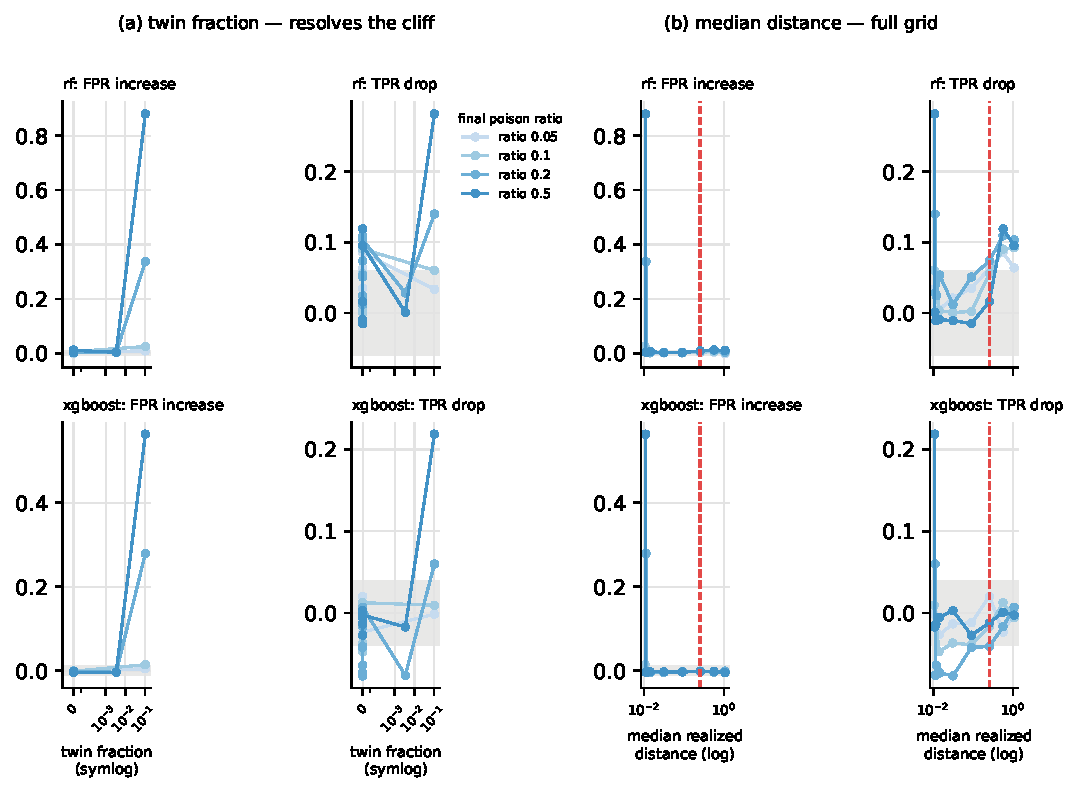
\includegraphics[width=\linewidth]{figures/F3_damage_vs_fidelity.pdf}
  % Source: results/phase0/loop/cicids/a1_damage_vs_fidelity.csv, s0_reference_damage.csv.
  % Regenerated by: python scripts/run.py figures --only F3  (experiments/paper_figures.py:fig_f3)
  \caption{TODO caption. A1 damage vs.\ realized mimicry distance to trusted benign (log scale),
  RF and XGBoost, fixed-threshold FPR and recalibrated-threshold TPR. Grey band: $\pm2\sigma$ of
  the control's own round-to-round variance. Dotted: S0 (genuine attacks) at the same ratio.}
  \label{fig:f3-damage-vs-fidelity}
\end{figure}

\begin{figure}[t]
  \centering
  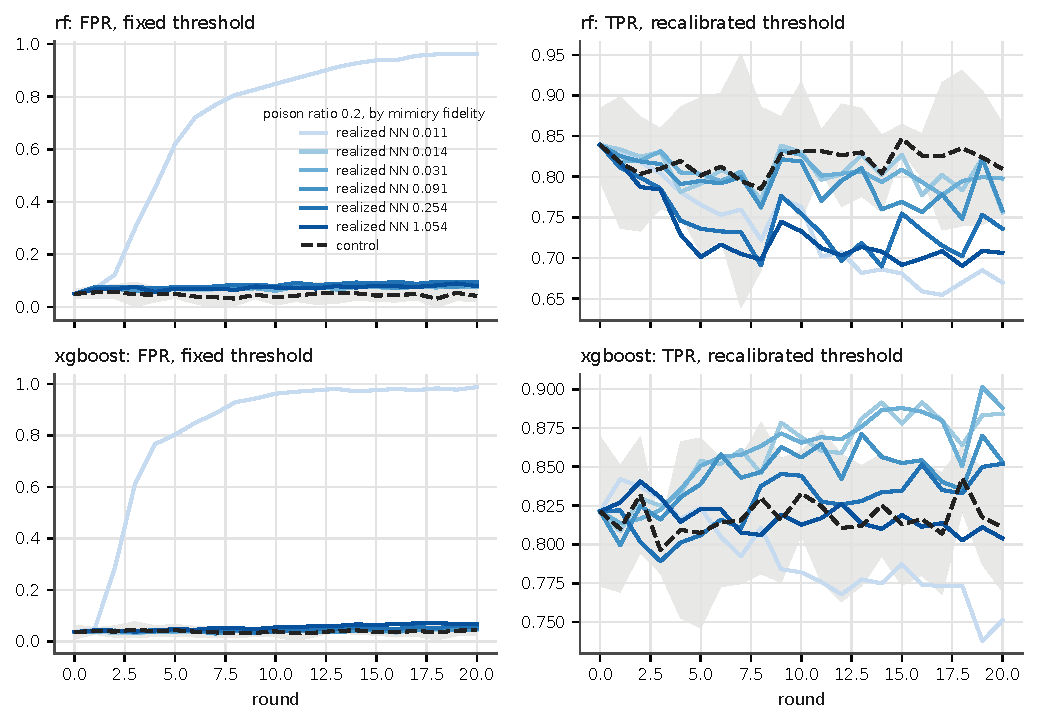
\includegraphics[width=\linewidth]{figures/F4_a1_trajectory.pdf}
  % Source: results/phase0/loop/cicids/jobs/*.csv (per-seed, per-round; undefended, tau=0).
  % Regenerated by: python scripts/run.py figures --only F4  (experiments/paper_figures.py:fig_f4)
  \caption{TODO caption. A1 on CICIDS2017 at poison ratio 0.2: per-round FPR (fixed threshold)
  and TPR (recalibrated threshold), by realized mimicry fidelity. Dashed: control mean
  $\pm2$\,sd across seeds.}
  \label{fig:f4-trajectory}
\end{figure}

\begin{figure}[t]
  \centering
  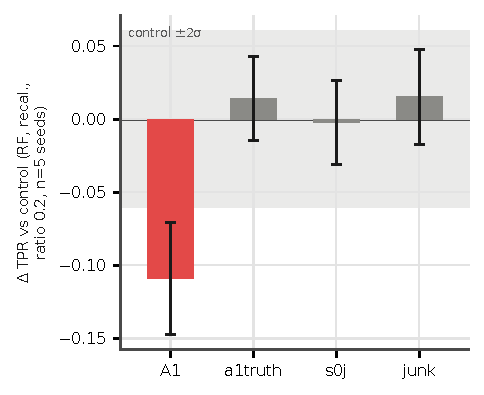
\includegraphics[width=\linewidth]{figures/F5_mechanism_isolation.pdf}
  % Source: results/phase0/export/summary.csv (rows: scenario in {a1,a1truth,s0j,junk},
  % model=rf, threshold_mode=recalibrated, target_poison_ratio=0.2, run_dir=cicids_recal).
  % Regenerated by: python scripts/run.py figures --only F5  (experiments/paper_figures.py:fig_f5)
  \caption{TODO caption. Mechanism isolation: $\Delta$TPR vs.\ control (RF, recalibrated
  threshold, ratio 0.2, $n=5$ seeds) for A1 and three null controls that each remove one
  candidate mechanism. Error bars: sd over seeds. Band: control's own $\pm2\sigma$.}
  \label{fig:f5-mechanism}
\end{figure}

\begin{table}[t]
  \centering
  \caption{TODO: the two channels. Source: DECISIONS.md s23 table.}
  \label{tab:two-channels}
  \begin{tabular}{lll}
    \toprule
    Channel & Model & Behavior \\
    \midrule
    FPR (false alarms) & RF, XGBoost & TODO \\
    TPR (detection loss) & RF only & TODO \\
    \bottomrule
  \end{tabular}
\end{table}
